% ====================================================================
%                                                                 
%
%       §01
%
%
% %%ts latex start%%[2019-03-07 Thu 14:45]%%ts latex end%%
% ====================================================================

% --------------------------------------------------------------------
% §21 Section <<Mengen und Familien>>
% --------------------------------------------------------------------
% --------------------------------------------------------------------
% §2.1 Subsection <<Motivation>>
% --------------------------------------------------------------------
\section{Mengen}
In diesem Abschnitt erweitern wir unser mathematisches Vokabular um den zentralen Begriff der \textit{Menge}, der im Vortrag über Logik bereits kurz eingeführt wurde (siehe \cref{mengenimlogikkapitel}). Die Idee ist sehr anschaulich: Wir möchten mehrere einzelne Objekte mit einer gemeinsamen Eigenschaft zu einem Ganzen zusammenfassen. So können wir beispielsweise die Zahlen $1,2,3,\dots$ in der \textit{Menge der natürlichen Zahlen} $\mathbb{N}$ zusammenfassen und als Gesamtheit betrachten.


\begin{de}[Cantorsche Mengendefinition\footnote{siehe \citet{Can1895}}]
Eine \textbf{Menge} $M$ ist eine Zusammenfassung bestimmter Objekte unserer Anschauung oder unseres Denkens zu einem Ganzen. Diese Objekte nennen wir die \textbf{Elemente} der Menge $M$. 
\end{de}

\begin{notion}
Wir haben folgende Möglichkeiten, eine Menge $M$ zu definieren: 
	\begin{itemize}
	\item Aufzählung der Elemente, z.B. $M = \{ \text{Antje, Bob, Charlie} \}$ oder $M = \{1, 2, 3, \ldots \}$. Für unendliche Mengen wie der letzteren kann diese Notation zu Unklarheiten führen und sollte dann eher vermieden werden. Geeigneter wäre:
	\item Definition über charakterisierende Eigenschaft, z.B. $M = \{ x \mid  x\text{ ist eine natürliche Zahl}\}$ (lies: Alle $x$, für die gilt: $x$ ist eine natürliche Zahl). (zuerst eingeführt in \cref{extension})
	\end{itemize}

Ist $m$ ein Element von $M$, d.h. tritt $m$ in einer solchen Aufzählung auf oder erfüllt die charakterisierende Eigenschaft einer Menge, so schreiben wir:
	\[m \in M \,.\]
Ist $m$ kein Element von $M$, so schreiben wir:
	\[m \notin M \,.\]
\end{notion}

\begin{bsp} Beispielsweise gilt
\begin{align*}
 23 & \in\{ x \mid  x\text{ ist eine Primzahl}\} \\
 \text{Dora} & \notin\{ \text{Antje, Bob, Charlie}\}
\end{align*}
\end{bsp}

\begin{notion}
	Um bequem Aussagen über die Elemente von Mengen zu treffen, nutzen wir folgende Schreibweisen:
	\begin{itemize}
		\item Um auszudrücken \glqq Für alle Elemente $m$ von $M$ gilt Eigenschaft $E$.\grqq\ schreiben wir
			\[ \forall m\in M: E(m) \,. \]
		\item Um auszudrücken \glqq Es gibt ein Element $m$ von $M$, das die Eigenschaft $E$ erfüllt.\grqq\ schreiben wir
			\[ \exists m\in M: E(m) \,. \]
	\end{itemize}	
\end{notion}

\begin{bsp} Es gilt:
\begin{align*}
 \forall m\in \Zz &:\ m^2 \geq 0 \\
 \exists m\in \Zz &:\ m^2=529
\end{align*}
\end{bsp}

Soweit die Erinnerung an die Einführung im Logikkapitel.


Um Mengen zu vergleichen, führen wir die folgenden neuen Begriffe ein:
\begin{de}\label{de:Mengenrelationen}
	Seien $M$ und $N$ zwei Mengen.
	\begin{itemize}
	\item Wir nennen $N$ eine \textbf{Teilmenge} von $M$, falls jedes Element von $N$ auch Element von $M$ ist:
		\[\forall n\in N: n\in M \,.\]
		Wir schreiben $N\subseteq M$.
		
		Wenn $N$ keine Teilmenge von $M$ ist, also wenn es ein Element von $N$, das kein Element von $M$ ist, gibt
			\[ \exists n\in N: n\notin M \,, \]
		so schreiben wir $N\nsubseteq M$. (Das ist gerade die Negation der obigen Aussage, siehe \cref{quantorennegieren} zur Negation des Allquantors.)
	\item Wir nennen $N$ eine \textbf{echte Teilmenge} von $M$, falls $N$ eine Teilmenge von $N$ ist, aber ein Element von $M$ existiert, dass kein Element von $N$ ist	
		\[N \subseteq M \wedge \exists m \in M: m \notin N \,.\]
		Wir schreiben $N\subsetneq M$.
		
		\begin{figure}[h]
			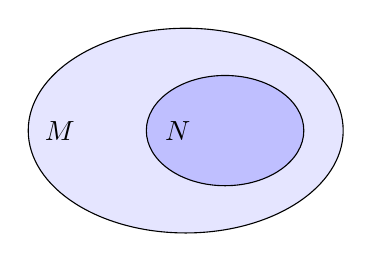
\begin{tikzpicture}
				\filldraw[fill=blue!10!white, draw=black] (0,0) ellipse (2cm and 1.3cm);
				\filldraw[fill=blue!25!white, draw=black] (.5,0) ellipse (1cm and .7cm);
				\path (-1.6,0) node {$M$} (-.1,0) node {$N$};
			\end{tikzpicture}
			\centering \caption{Die Menge $N$ ist (echte) Teilmenge der Menge $M$.}
		\end{figure}
		
	\item $M$ und $N$ heißen \textbf{gleich}, falls sie die gleichen Elemente haben
		\[ \forall x: (x\in M\Leftrightarrow x\in N) \,.\]
		Wir schreiben $M=N$.\footnote{In der formalen Mengenlehre muss diese Eigenschaft axiomatisch gefordert werden, siehe \href{https://de.wikipedia.org/wiki/Extensionalit\%C3\%A4tsaxiom}{Extensionalitätsaxiom}.}
	\end{itemize}
	Bisweilen werden in der Literatur auch abweichende Notationen benutzt: etwa $N\subseteq M$ für beliebige und $N\text{ \reflectbox{$\supset$} }M$ für echte Teilmengen; oder aber $N\text{ \reflectbox{$\supset$} }M$ für beliebige und $N\subsetneqq M$ für echte Teilemengen. Die Lehre ist, am besten verlässt man sich für die Angabe von echten Teilmengen nicht nur auf Symbole und gibt auch in Worten an, was gemeint ist.
	
	Eine weitere Verwechslungsgefahr verbirgt sich jetzt in (sprachlichen) Ausdrücken wie \glqq ... ist in ... enthalten\grqq\,. Per se ist nicht immer klar, ob enthalten sein als Teilmenge $A\subset M$ oder als Element $A\in M$ gemeint ist. Wenn die Unterscheidung aus dem Kontext nicht ersichtlich ist, sollte man daher explizit \glqq als Teilmenge ... enthalten\grqq\, oder \glqq ist Element von ...\grqq\, schreiben.
\end{de}

\begin{bsp}\quad
	\begin{itemize}
		\item Es ist $\{\text{Zarah, Torben}\}\subsetneq\{\text{Zarah, Torben, John}\}$.
		\item Es gilt $\mathbb{Z}\nsubseteq\mathbb{N}$, etwa ist $-1\in\mathbb{Z}$, aber $-1\notin\mathbb{N}$.
	\end{itemize}
\end{bsp}

\begin{sat}[Eigenschaften der Mengeninklusion]\label{sat:Mengenrelationen}
Seien $L, N, M$ Mengen. Dann gilt:
	\begin{enumerate}[a)]
		\item $M\subseteq M$ (Reflexivität).
		\item Aus $M \subseteq N$ und $N\subseteq M$ folgt $M=N$ (Antisymmetrie).
		\item Aus $L\subseteq N$ und $N\subseteq M$ folgt $L\subseteq M$ (Transitivität).
	\end{enumerate}
\end{sat}

\begin{figure}[h]
	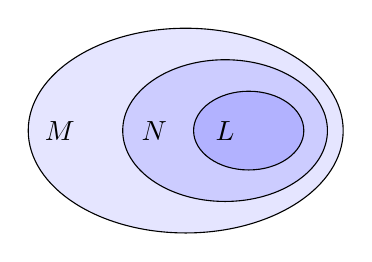
\begin{tikzpicture}
		\filldraw[fill=blue!10!white, draw=black] (0,0) ellipse (2cm and 1.3cm);
		\filldraw[fill=blue!20!white, draw=black] (.5,0) ellipse (1.3cm and .9cm);
		\filldraw[fill=blue!30!white, draw=black] (.8,0) ellipse (.7cm and .5cm);
		\path (-1.6,0) node {$M$} (-.4,0) node {$N$} (.5,0) node {$L$};
	\end{tikzpicture}
	\centering \caption{Illustration der Transitivität}
\end{figure}

\begin{bew}
	\begin{enumerate}[a)]
		\item Für alle Elemente $m\in M$ gilt per se schon $m\in M$, also ist $M$ in $M$ enthalten. (Siehe auch \cref{AtoA}: Jede Aussage impliziert sich selbst.)
		\item Zu zeigen ist, dass $M$ und $N$ die selben Elemente haben, also die Äquivalenz aus \cref{de:Mengenrelationen} (c). Wir tun dies, indem wir erst Hin- und dann Rückrichtung zeigen (vgl. \cref{hinruck}). Sei $x$ ein beliebiges Objekt. Ist $x$ ein Element in $M$, so folgt wegen $M\subseteq N$ schon $x\in N$. Ist umgekehrt $x$ ein Element in $N$, so folgt wegen $N\subseteq M$ schon $x\in M$. Damit sind beide Richtungen gezeigt und wir sind fertig.
		\item Sei $x\in L$ ein Element. Wegen $L\subseteq N$ gilt dann $x\in N$. Aus $x\in N$ folgt wegen $N\subseteq M$ dann $x\in M$. (Das war ein direkter Beweis mit Zwischenschritten, vgl. \cref{zwischenschritt}) \qed
        \[ x\in L\xrightarrow{L\subseteq N} x\in N \xrightarrow{N\subseteq M} x\in M \]
	\end{enumerate}
\end{bew}

\begin{bem}
	Eigenschaft (ii) liefert uns den üblichen Weg, Gleichheit zweier Mengen zu zeigen; bestehend aus zwei Schritten:
		\begin{enumerate}
			\item[$M\subseteq N$:] Beginne mit einem beliebigen Element\footnote{Da es sich bei „$M\subseteq N$“ um eine Allaussage handelt (\emph{jedes} Element von $M$ ist ein Element von $N$), leitet sich diese Beweistechnik aus \cref{allbeweis} ab.} $m\in M$ und folgere, dass $m$ in $N$ liegen muss (also die charakterisierende Eigenschaft erfüllt oder als Element gelistet ist).
			\item[$M\supseteq N$:] Beginne mit einem beliebigen Element $n\in N$ und folgere, dass $n$ in $M$ liegen muss.
		\end{enumerate}
	Sind diese Eigenschaften erfüllt, folgt aus unserem Satz $M=N$.
\end{bem}

\begin{bsp}\label{bsp:mengengleichheiten} Es gilt:
	\begin{enumerate}[a)]
		\item $\{x\in\Nz\mid x\text{ ist prim und gerade}\}=\{2\}$.
\begin{bew}
		\begin{itemize}			
		\item[$\glqq\subseteq\grqq$] Sei $x$ in der linken Seite enthalten, also eine gerade Primzahl. Dann ist $x$ durch 2 teilbar, da $x$ gerade ist. Da $x$ Primzahl ist, kann $x$ aber nur durch 1 und sich selbst teilbar sein und es folgt $x=2$, also $x\in\{2\}$.
		\item[$\glqq\supseteq\grqq$] Ist umgekehrt $x\in\{2\}$, also $x=2$, so ist $x$ eine gerade ganze Zahl sowie eine Primzahl, also in der linken Seite enthalten.		
		\end{itemize}
\end{bew}
		\item $\{1,2,3\}=\{1,1,3,2\}$.
\begin{bew}
		\begin{itemize}			
			\item[$\glqq\subseteq\grqq$] Sei $x\in\{1,2,3\}$, also $x=1$, $x=2$ oder $x=3$. In jedem dieser Fälle\footnote{vgl. \cref{fallunterscheidung}} gilt auch $x\in\{1,1,3,2\}$.
			\item[$\glqq\supseteq\grqq$] Sei umgekehrt $x\in\{1,1,3,2\}$,  also $x=1$, $x=1$, $x=3$ oder $x=2$. In jedem dieser Fälle gilt auch $x\in\{1,2,3\}$.
		\end{itemize}
\end{bew}
	\end{enumerate}
\end{bsp}


\begin{bem}\label{mengen:strukturlos}
	Im letzten Beispiel sehen wir ganz deutlich, dass die Elemente einer Menge keiner Reihenfolge oder \glqq Zählung\grqq\ unterliegen: Eine Menge trägt von sich aus bis auf die Angabe ihrer Elemente bzw. charakterisierenden Eigenschaft keine weitere Struktur; Fragen wie \glqq Wie genau / Wie oft / An welcher Stelle ist $m$ in $M$ enthalten?\grqq\ kann sie also nicht beantworten, sondern nur \glqq Ist $m$ in $M$ enthalten, oder ist $m$ nicht in $M$ enthalten?\grqq .
\end{bem}




\begin{de}
	Die Menge, die keine Elemente enthält, bezeichnen wir als die \textbf{leere Menge}, geschrieben $\emptyset$. In Anlehnung an die Notation durch Aufzählung aller Elemente schreiben manche Autoren auch $\{\}$. Die leere Menge lässt sich auch als Extension einer Eigenschaft, die kein einziges Objekt besitzt, realisieren. Beispielsweise ist
		\[ \emptyset = \{ x \mid x\neq x\} \]
\end{de}

\begin{bem}[\textbf{Die} leere Menge]
	Wir können tatsächlich von \textit{der} leeren Menge sprechen: Ist $A$ eine weitere Menge ohne Elemente, so haben $A$ und $\emptyset$ die gleichen Elemente (nämlich keine) und nach Definition der Mengengleichheit \cref{de:Mengenrelationen} folgt $A=\emptyset$.
\end{bem}

\begin{bsp}
	Es gilt
		\[ \{ x \mid x \text{ ist eine gerade Primzahl mit } x\neq 2 \} = \emptyset \,. \]
	Dazu müssen wir zeigen, dass für alle $x$ die Aussage \glqq$x$ ist eine gerade Primzahl mit $x\neq 2$\grqq\, eine falsche Aussage ist.
	
	Beweis per Widerspruch: Angenommen, $x$ wäre ein Element der linken Menge. Dann wäre $x$ eine gerade Primzahl. Wir haben oben gesehen, dass 2 die einzige gerade Primzahl ist, es müsste also $x=2$ gelten. Aber $x\neq2$ gilt nach Voraussetzung und wir erhalten einen Widerspruch. Daher kann die linke Menge keine Elemente enthalten und ist gleich der leeren Menge. 
\end{bsp}

\begin{bem}[Mengen von Mengen von Mengen von \dots]
Sei $A$ eine Menge. Das Konzept der Menge ist iterativ. Eine Menge kann wiederum Element einer anderen Menge sein, die wiederum in einer Menge enthalten sein kann. Zum Beispiel ist $A$ Element der Menge $\{A\}$, die wiederum ein Element von $\{ \{A\}\}$ ist usw. Wichtig sich klar zu machen, ist der Unterschied zwischen $A$ und $\{A\}$, also der Menge $A$ und derjenigen Menge, die nur das Element $A$ enthält. Betrachte etwa $\emptyset$ im Vergleich mit $\{\emptyset\}$. Auch wenn es zunächst scheinen mag, dass in beiden Objekten letztlich \glqq nichts drin ist\grqq\,, so liegen doch sehr verschiedene Objekte vor. Mit $\emptyset$ haben wir nämlich die Menge mit keinen Elementen, und mit $\{\emptyset\}$ eine einelementige Menge, deren einziges Element $\emptyset$ ist. Eine mögliche mengentheoretische Konstruktion der Natürlichen Zahlen macht sich genau diesen Unterschied zu Nutze.\footnote{Siehe \href{https://de.wikipedia.org/wiki/Nat\%C3\%BCrliche\_Zahl\#Von\_Neumanns\_Modell\_der\_nat\%C3\%BCrlichen\_Zahlen}{von Neumann Konstruktion}.}
\end{bem}

\begin{bem}[Vacuous Truth]\label{vacuoustruth}
	Eine weitere Feinheit im Umgang mit leeren Mengen sind so genannte \glqq Vacuous Truths\grqq\,. Das sind Aussagen wie
		\begin{itemize}
			\item \glqq Alle rosa Elefanten können fliegen.\grqq
			\item \glqq Alle meine Geschwister sind Gürteltiere\grqq, gesprochen von einem Einzelkind.
		\end{itemize}	
	Formal sind diese Aussagen von der Form
		\[ \forall x\in M:E(x) \,, \]
	wobei $E$ in unserem Fall die Eigenschaft \glqq kann fliegen\grqq\, bzw. \glqq ist ein Gürteltier\grqq\, war, und $M$ die Menge der rosa Elefanten bzw. der Geschwister des Einzelkindes war. Diese Mengen haben keine Elemente, sind also gleich der leeren Menge:
		\[ \forall x\in \emptyset:E(x) \,. \]
	Wenn wir uns nun erinnern, was diese Kurzschreibweise in \cref{boundedquant} hieß, können wir auch schreiben
		\[ \forall x: \left(x\in \emptyset\implies E(x)\right) \,. \]
	Die Aussage $x\in\emptyset$ ist aber für alle Objekte $x$ falsch, denn die leere Menge hat keine Elemente. Nach dem Prinzip \textit{ex falso quod libet} aus \cref{exfalso} ist die Aussage $x\in \emptyset\implies E(x)$ also für jedes $x$ war, und somit auch $\forall x: \left(x\in \emptyset\implies E(x)\right)$ eine wahre Aussage.
	
	Wir lernen: Aussagen, die den Elementen einer leeren Menge (wie der Menge der rosa Elefanten oder den Geschwistern eines Einzelkindes) eine gewisse Eigenschaft zuordnen, sind immer wahr, egal was die Eigenschaft ist.
\end{bem}

Ein weiteres Beispiel für eine vacuous truth ist der folgende Satz:

\begin{sat}\label{emptyinall}
	Die leere Menge $\emptyset$ ist Teilmenge jeder beliebigen Menge.
\end{sat}

\begin{bew}
	Sei $M$ eine beliebige Menge. Zu zeigen ist $\emptyset\subseteq M$, also
		\[ \forall x\in\emptyset: x\in M \,.\]
	Ausgeschrieben ist das 
		\[ \forall x: \left(x\in \emptyset\implies x\in M\right) \,, \]
	was nach \textit{ex falso quod libet} eine wahre Aussage ist. 
	
	Anschaulich ergibt das auch Sinn: Die Forderung, dass jedes Element der Menge $\emptyset$ (die keine Elemente hat) in $M$ enthalten ist, ist leicht zu erfüllen. \qed
\end{bew}



%------------------
% Def. Potenzmenge
\begin{de} \label{powerset}
	Die \textbf{Potenzmenge} einer Menge $M$ ist die Menge aller Teilmengen von $M$:
	\begin{align*}
		\cP(M) := \{N \mid N \subset M\}
	\end{align*}
	Es gilt stets $\emptyset \in \cP(M)$ und $M \in \cP(M)$, da $\emptyset \subset M$ und $M \subset M$ nach \cref{emptyinall} und \cref{sat:Mengenrelationen}a) immer wahr ist.
\end{de}

\begin{bsp}
	Sei $M=\{1,2,3\}$. Dann ist
		\[ \cP(M)=\left\{\emptyset,\{1\},\{2\},\{3\},\{1,2\},\{1,3\},\{2,3\},\{1,2,3\}\right\}\,. \]
\end{bsp}


In alten Büchern wird die Potenzmenge einer Menge $X$ auch mit „$2^X$“ notiert, woher auch der Name „Potenzmenge“ stammt. Der folgende Satz erklärt, warum:
\begin{sat}[Name der Potenzmenge]
	Seien $M$ eine Menge und $n\in\Nz$ eine natürliche Zahl. Hat $M$ genau $n$ Elemente, so hat $\cP(M)$ genau $2^n$ Elemente.
\end{sat}

\begin{bew}
	Wir verallgemeinern, was wir eben im Beispiel gesehen haben: Wir können eine Teilmenge $N$ von $M$ konstruieren, indem wir für jedes Element $m\in M$ entscheiden, ob es in $N$ enthalten sei oder nicht. Dies sind $n$ Entscheidungen zwischen je zwei Möglichkeiten, nämlich eine Entscheidung für jedes Element $m\in M$. Jede Teilmenge von $M$ kann auf diese Weise konstruiert werden, und unterschiedliche Wahlen schon bei einer einzigen der $n$ Entscheidungen ergeben verschiedene Teilmengen $N$, also gibt es $2^n$ Teilmengen von $M$. \qed
\end{bew}

% --------------------------------------------------------------------
% §2.4 Subsection <<Familien>>
% --------------------------------------------------------------------
\section{Familien}
Unser Begriff der Menge ist schon sehr mächtig, greift --- wie vorhin gesehen -- in manchen Fällen jedoch noch zu kurz.

Mit dem Begriff der Familie möchten wir nun einer Sammlung von Objekten eine zusätzliche Struktur verleihen: Statt uns nur zu merken, welche Objekte in unserer Sammlung enthalten sind, unterscheiden wir nun verschiedene \glqq Stellen\grqq\,, an denen Objekte in der Sammlung sitzen können. Realisiert wird das, indem wir die Elemente unserer Sammlung mit Indizes versehen und dann vom Objekt an Index/Stelle $i$ sprechen:

\begin{de}[Familien]
	Eine \textbf{Familie} $(a_i)_{i\in I}$ ist eine Sammlung von Objekten $a_i$ indiziert über eine Menge $I$. Soll heißen: An jedem Index $i$ sitzt ein Objekt $a_i$.
	
	Die Menge $I$ wird die \textbf{Indexmenge} der Familie genannt. (Dieser Name suggeriert häufig, dass die Menge $I$ irgendeine besondere Eigenschaft haben müsste. Tatsächlich kann aber jede beliebige Menge als Indexmenge dienen und der Name bezeichnet eher die Rolle, die die Menge in der Konstruktion spielt.) Wenn wir sowas wie „Sei $(a_i)_{i\in I}$ eine Familie“ schreiben, so meinen wir damit „Sei $I$ eine beliebige Menge und $(a_i)_{i\in I}$ eine Familie mit Indexmenge $I$“.
\end{de}



\begin{de} \label{familie}
 Sei $(a_i)_{i\in I}$ eine Familie. Ist $A$ irgendeine Menge, sodass jedes der $a_i$'s ein Element von $A$ ist, so nennt man die Familie $(a_i)_{i\in I}$ eine \textbf{(durch $I$ indizierte) Familie mit Einträgen aus $A$} oder auch eine \textbf{$A$-wertige Familie}. \\
 Die Menge aller Familien mit Indexmenge $I$ und Einträgen aus $A$ wird mit $A^I$ notiert:
 \[ A^I := \{ (a_i)_{i\in I} \mid \forall i\in I:\ a_i \in I \} \]
 Manchmal nennt man $A^I$ die „$I$-te Potenz von $A$“, was aber nicht mit der Potenzmenge aus \cref{powerset} verwechselt werden sollte.
\end{de}


\begin{bsp}
	\begin{enumerate}[a)]
	\item Nehmen wir als Indexmenge $I$ die Menge der Stühle im Raum und als das Objekt $a_i$ die Person, die auf Stuhl $i$ sitzt, so erhalten wir eine Familie der hier im Raum sitzenden Leute $(a_i)_{i\in I}$. Sie unterscheidet sich von der \textit{Menge} der hier im Raum sitzenden Leute dadurch, dass wir auch wissen, wer auf welchem Stuhl sitzt.
	
	\item Es ist $\Qz^\Nz$ die Menge all derjenigen Familien, deren Indexmenge $\Nz$ ist und deren Einträge allesamt rationale Zahlen sind. Eine solche Familie ist beispielsweise $(a_n)_{n\in\mathbb{N}}$ mit $a_n:=\frac{1}{n}$.
		\begin{figure}[h]
			\centering
			\begin{tabular}{c|cccc}
				$n$ & 1 & 2 & 3 & $\dots$ \\ \midrule
				$a_n$ & 1 & 1/2 & 1/3 & $\dots$
			\end{tabular}
		\end{figure}
Familien, deren Indexmenge die Menge $\Nz$ der natürlichen Zahlen ist, heißen \emph{Folgen} und sind ein zentrales Thema im sechsten Vortrag.\footnote{siehe \cref{folge}}
	\item ($*$) Für Informatiker: Arrays sind vom Konzept her Familien. Indexmenge ist meist
		\[ \{0,1,\ldots,k_1\}\times\dots\times\{0,1,\dots,k_n\} \,,\]
		wobei $n$ die Dimension des Arrays ist und $k_i$ die Länge des Arrays in Dimension $i$.
	\end{enumerate}
\end{bsp}


\begin{bsp}
	Das unendliche Produkt
		\[ \mathbb{R}^\mathbb{N}=\prod_\mathbb{N}\mathbb{R} \]
	besteht aus unendlichen Familien der Form
		\[ (a_1,a_2,a_3,\dots)\,, \]
	wobei die $a_i$ reelle Zahlen sind. Man spricht von \emph{reellen Zahlenfolgen}. Im Kapitel über Folgen werden uns diese Objekte namensgebend wieder begegnen.
\end{bsp}

\begin{de}[Gleichheit von Familien] \label{gleichheit:familien}
	Zwei Familien $(a_i)_{i\in I}$ und $(b_i)_{i\in I}$ mit der selben Indexmenge $I$ heißen \textbf{gleich}, wenn sie an jeder Stelle $i\in I$ den gleichen Eintrag haben:
		\[ \forall i\in I: a_i=b_i \,. \]
\end{de}

\begin{bsp}
	Tauschen zwei Studierende ihre Sitzplätze $i$ und $j$, so wird aus der Familie $(a_i)_{i\in I}$ der im Raum sitzende Leute eine neue Familie $(b_i)_{i\in I}$. Diese Familien sind nicht gleich, denn es gilt $a_i\neq b_i$ und $a_j\neq b_j$. Betrachten wir nur die simple \textit{Menge} der im Raum sitzenden Leute, so verändert sie sich durch den Sitzplatzwechsel nicht, denn sie hat vorher wie nachher dieselben Elemente. 
\end{bsp}

\begin{bem}[Mengen vs. Familien]
	Das Beispiel macht den Unterschied zwischen den Begriffen der Familie und der Menge noch einmal sehr deutlich. Zwei Mengen, in denen die gleichen Elemente vorkommen, sind schon gleich; für eine Gleichheit von Familien müssen die Elemente aber gerade an den entsprechenden Indizes übereinstimmen. Im Gegensatz zu Mengen haben Familien also eine gewisse Struktur auf ihren Elementen, gegeben durch die Indizierung. Vergleiche \cref{mengen:strukturlos}.
\end{bem}

\begin{de}[Tupel]
	Sei $n\in \Nz$. Familien $(a_i)_{i\in I}$ mit Indexmengen der Form $I=\{1,2,\dots,n\}$ nennt man auch \textbf{$n$-Tupel} und schreibt
		\[ (a_1,a_2,\dots,a_n) \,. \]
	2-Tupel, also Objekte der Form $(a,b)$, nennt man auch (geordnete) \textbf{Paare}, 3-Tupel nennt man auch \textbf{Tripel}. \\[0.5em]
	Ist $A$ eine Menge, so notiert man die Menge aller $n$-Tupel mit Einträgen aus $A$ mit $A^n$:
	\[ A^n := \{ (a_1,\dots , a_n) \mid a_1,\dots , a_n \in A \} \]
\end{de}


\begin{bsp}
 Es ist $\Rz^3$ die Menge aller Tripel reeller Zahlen:
 \[ \Rz^3 = \{(x,y,z) \mid x,y,z\in \Rz \} \]
 Diese Menge ist dir vielleicht schon aus der Schule als „dreidimensionaler Raum“ bekannt. In der Geometrie repräsentieren die Elemente des $\Rz^3$ Punkte im Raum und die drei Einträge eines solchen Tripels repräsentieren seine Koordinaten in einem Koordinatensystem.
\end{bsp}



\begin{bem}[Gleichheit von Tupeln]
	Um die Gleichheit von Familien noch einmal zu konkretisieren: Nach \cref{gleichheit:familien} sind zwei $n$-Tupel $(a_1,\dots,a_n)$ und $(b_1,\dots,b_n)$ genau dann gleich, wenn $a_1=b_1$, $a_2=b_2$, $\dots$ und $a_n=b_n$ gilt.
\end{bem}

\begin{bsp}[Mengen vs. Familien]
	In \cref{bsp:mengengleichheiten} hatten wir gesehen, dass die Mengengleichheit $\{1,2,3\}=\{1,1,3,2\}$ gilt. Betrachten wir stattdessen die Tupel $(1,2,3)$ und $(1,1,3,2)$, so liegen zwei sehr unterschiedliche Objekte vor, denn schon die Indexmengen der Familien sind verschieden (die eine Familie ist ein 3-Tupel, die andere ein 4-Tupel). Doch auch wenn wir die 3-Tupel $(1,2,3)$ und $(1,3,2)$ vergleichen würden, wären sie nicht gleich, denn sie unterscheiden sich an zweiter und dritter Stelle. Dagegen sind $\{1,2,3\}$ und $\{1,3,2\}$ dieselbe Menge. Bei einer bloßen Mengen gibt es keine „zweite Stelle“ oder dergleichen.
\end{bsp}

\begin{bem}[Mengen aus Familien gewinnen] \label{mengeeinerfamilie}
	Gegeben eine \textit{Familie} $(a_i)_{i\in I}$ können wir stets die \textit{Menge} der Einträge der Familie $\{a_i\mid i\in I\}$ aufstellen und \glqq vergessen\grqq\, dabei einfach die zusätzliche Struktur. Diese Objekte sollte man nicht verwechseln!
	
	Betrachten wir noch einmal die Familie $(a_i)_{i\in I}$ der im Raum sitzenden Leute, so ist $\{a_i\mid i\in I\}$ nur noch die \textit{Menge} der im Raum sitzenden Leute und wir vergessen, wer wo sitzt.
\end{bem}



% --------------------------------------------------------------------
% §2.2 Subsection <<Mengen-Bastelstunde>>
% --------------------------------------------------------------------
\section{Mengen-Bastelstunde}
Wir beschäftigen uns jetzt mit Operationen, die wir auf Mengen anwenden können, um aus mehreren Mengen neue Mengen zu generieren.

%%% Wie rechtsbuendig?
\begin{de}
	Seien $A, B$ zwei Mengen. Wir definieren:
	\begin{itemize}
		\item den \textbf{Schnitt} von $A$ und $B$: 
\begin{align*}
 A \cap B & := \{x \mid x \in A \wedge x \in B\} && (\text{lies: „$A$ geschnitten $B$“})
\end{align*}

			
			\begin{figure}[h]
				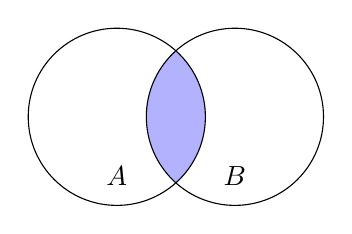
\begin{tikzpicture}[scale=.75]
					\begin{scope}
						\clip (-1,0) circle (1.5cm);
						\fill[blue!30!white] (1,0) circle (1.5cm);
					\end{scope}
				\draw (-1,0) circle (1.5cm) (-1,-1) node {$A$} (1,0) circle (1.5cm) (1,-1) node {$B$};
				\end{tikzpicture}
				\centering \caption{Schnitt zweier Mengen $A$ und $B$}
			\end{figure}
		
		
		\item die \textbf{Vereinigung} von $A$ und $B$:
\begin{align*}
 A \cup B & := \{x \mid x \in A \vee x \in B\} && (\text{lies: „$A$ vereinigt $B$“})
\end{align*}
			
			\begin{figure}[h]
				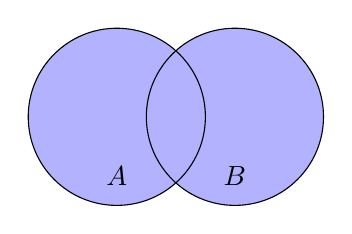
\begin{tikzpicture}[scale=.75]
					\filldraw[fill=blue!30!white, draw=black] (-1,0) circle (1.5cm) (-1,-1) node {$A$} (1,0) circle (1.5cm) (1,-1) node {$B$};
				\end{tikzpicture}
				\centering \caption{Vereinigung zweier Mengen $A$ und $B$}
			\end{figure}
		
		\item das \textbf{kartesische Produkt} von $A$ und $B$: 
\begin{align*}
 A \times B & := \left\{ (a,b) \mid a\in A, b\in B \right\}  && (\text{lies: „$A$ kreuz $B$“})
\end{align*}
		
			Dabei sind die Elemente $(a,b)$ des kartesischen Produkts genau diejenigen Paare, deren erster Eintrag in $A$ und deren zweiter Eintrag in $B$ liegt.
			
			\begin{figure}[h]
				\begin{tikzpicture}
					\draw[style=help lines,step=1 cm] (-2.3,-2.3) grid (1.5,1.5);
					\begin{scope}
						\draw[->, thick] (-2.5,-2) -- (2,-2) node[right] {$A$};
						\draw[->, thick] (-2,-2.5) -- (-2,2) node[above] {$B$};
					\end{scope}
				\end{tikzpicture}
				\centering \caption{Das \textit{kartesische} Produkt hat seinen Namen aus dieser Darstellung als Ebene mit kartesischen „Koordinatenachsen“ $A$ und $B$.}
			\end{figure}
		
		\item das \textbf{Komplement} von $B$ in $A$ oder auch die \textbf{Differenzmenge} von $A$ und $B$: 
\begin{align*}
A \setminus B & := \{ x \in A \mid x \notin B \}  && (\text{lies: „$A$ ohne $B$“})
\end{align*}
			Manche Autoren schreiben auch $A-B$.
			
			\begin{figure}[h]
				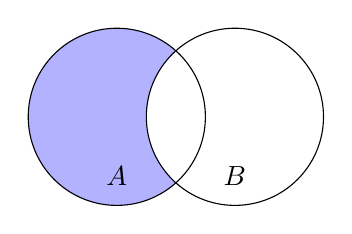
\begin{tikzpicture}[scale=.75]
					\fill[blue!30!white] (-1,0) circle (1.5cm);
					\begin{scope}
						\clip (-1,0) circle (1.5cm);
						\fill[white] (1,0) circle (1.5cm);
					\end{scope}
					\draw (-1,0) circle (1.5cm) (-1,-1) node {$A$} (1,0) circle (1.5cm) (1,-1) node {$B$};
				\end{tikzpicture}
				\centering \caption{Komplement der Menge $B$ in der Menge $A$}
			\end{figure}
		
	\end{itemize}
	Ist allgemeiner eine Familie von Mengen $(M_i)_{i\in I}$ gegeben, so definiert man
		 \begin{align*}
		 	\bigcap_{i\in I} M_i&:= \{x \mid \forall i\in I: x\in M_i\}\,,\\
		 	\bigcup_{i\in I}M_i&:= \{x \mid \exists i\in I: x\in M_i\}\,,\\
		 	\prod_{i\in I}M_i&:=\{ \text{Familien } (x_i)_{i\in I} \mid \forall i\in I: x_i\in M_i\}\,. 
		 \end{align*}
	 Ist die Indexmenge von der Form $I=\{1,2,\dots,n\}$, so setzt man meistens die für zwei Mengen eingeführte Notation mit kleinen Zeichen fort und schreibt
	 	\begin{align*}
	 		\bigcap_{i\in I} M_i&=: \bigcap_{i=1}^n M_i =: M_1\cap M_2\cap\dots\cap M_n \\
	 		\bigcup_{i\in I} M_i&=: \bigcup_{i=1}^n M_i =: M_1\cup M_2\cup\dots\cup M_n \\
	 		\prod_{i\in I} M_i&=: \prod_{i=1}^n M_i =: M_1\times M_2\times\dots\times M_n 
	 	\end{align*}
	Zwei Mengen $A,B$ heißen \textbf{disjunkt}, wenn sie keine gemeinsamen Elemente haben, also $A\cap B=\emptyset$ gilt.
\end{de}

\begin{bem}[Mengen-Operatoren und Aussagen-Operatoren]
	Wie man vielleicht auch in den Definitionen erkennt, sind die Zeichen $\cap$ und $\cup$ an denen für die logischen Verknüpfungen $\wedge$ und $\vee$ angelehnt. Man sollte diese Zeichen trotzdem sauber unterscheiden: Die Formel $M\cap N$ ergibt nur Sinn, wenn $M$ und $N$ Mengen sind; die Formel $A\wedge B$ nur, wenn $A$ und $B$ Aussagen sind. $M\wedge N$ für zwei Mengen $M, N$ ist kein sinnbehafteter Ausdruck!
	
	Bis auf das Produkt kann man für jede Mengenoperation solche schönen Analogien zu den Logiksymbolen ziehen, um sie sich besser zu merken:

	\begin{figure}[h]
		\centering
		\begin{tabular}{c|c|c|c|c|c}
		Mengenoperation & $M\cap N$ & $M\cup N$ & $M\setminus N$ & $\bigcap_{i\in I} M_i$ & $\bigcup_{i\in I} M_i$ \\ \midrule
		Logiksymbol & $\land$ & $\lor$ & $\neg$ & $\forall$ & $\exists$
		\end{tabular}
		\caption{Mengen- und Logiksymbole im Vergleich}
	\end{figure}
\end{bem}

\begin{bsp}
	Sei $ A = \{1, 2, 4\}, \ B = \{1, 4, 7\}$. Dann gilt: 
	\begin{itemize}
		\item $A \cap B = \{1, 4\}$, insbesondere sind $A$ und $B$ nicht disjunkt.
		\item $A \cup B = \{1, 2, 4, 7\}$
		\item $A\times B = \left\{ (1,1),(1,4),(1,7),(2,1),(2,4),(2,7),(4,1),(4,4),(4,7) \right\}\,.$		
		\item $A \setminus B = \{2\}$
	\end{itemize}
\end{bsp}

\begin{bsp}
	Sei $I=\mathbb{N}_0$ unsere Indexmenge. Zu $n\in\mathbb{N}_0$ definieren wir
	\[ M_n := \{ x\in\mathbb{Z} \mid x\text{ teilt } n \} \,.\]
	Dabei soll $x$ teilt $n$ heißen, dass es eine ganze Zahl $c\in\Zz$ gibt mit $c\cdot x=n$.
	
	Dann gilt 
	\begin{enumerate}[a)]
		 \item $\bigcap_{n\in\mathbb{N}_0} M_n= \{x\in \mathbb{Z} \mid \forall n\in \mathbb{N}_0:x\in M_n\}= \{x\in \mathbb{Z} \mid \forall n\in \mathbb{N}_0: x\text{ teilt }n\}$.
		 
		 Wir behaupten nun:
		 	\[\forall n\in\Nz_0:x\text{ teilt }n \quad\Longleftrightarrow\quad (x=1)\vee (x=-1) \,.\]
\begin{bew}	
			 \begin{itemize}
			 	\item[\glqq$\Rightarrow$\grqq] Aus $\forall n\in\Nz_0:(x\text{ teilt }n )$ folgt insbesondere $x$ teilt 1, wenn wir $n=1$ setzen. Die einzigen Teiler von 1 in $\Zz$ sind aber $1$ und $-1$.
			 	\item[\glqq$\Leftarrow$\grqq] Sei umgekehrt $n\in\Nz_0$ beliebig und $x=1$ bzw. $x=-1$. Dann ist $x\cdot n=n$ bzw. $x\cdot (-n)=n$ und $x$ teilt daher $n$. \qed
			 \end{itemize}
\end{bew}
		 Daher gilt 
		 	$$\bigcap_{n\in\mathbb{N}_0} M_n=\{x\in \mathbb{Z} \mid \forall n\in \mathbb{N}_0: x\text{ teilt }n\}=\{1,-1\}\,.$$
		 \item $\bigcup_{n\in\mathbb{N}_0} M_n= \{x\in \mathbb{Z} \mid \exists n\in \mathbb{N}_0:x\in M_n\}= \{x\in \mathbb{Z} \mid \exists n\in \mathbb{N}_0: x\text{ teilt }n\}$.
		 
		  Wir behaupten nun:
		 \[\bigcup_{n\in\mathbb{N}_0} M_n = \Zz\]
    \begin{bew} \begin{itemize}
                 \item[„$\subseteq$“:] Da jedes der $M_n$'s eine Teilmenge von $\Zz$ ist, ist insgesamt auch $\bigcup_{n\in \Nz_0} M_n$ eine Teilmenge von $\Zz$.
                 \item[„$\supseteq$“:] Sei $x\in\Zz$ beliebig. Ist $0\leq x$, so gilt $x\in\Nz_0$ und $1\cdot x=x$, also teilt $x$ eine natürliche Zahl (sich selbst). Ist $x\leq 0$, so gilt $-x\in\Nz_0$ und $-1\cdot x= -x$, also teilt $x$ eine natürliche Zahl (nämlich $-x$). In jedem Fall teilt $x$ eine natürliche Zahl, sodass $x\in \bigcup_{n\in \Nz_0} M_n$. \qed
                \end{itemize}
\end{bew}
	\end{enumerate}
\end{bsp}






\begin{bem}[disjunkte Vereinigung]
	Möchte man exakt zwei \glqq Kopien\grqq\, einer Menge (etwa $\mathbb{N}$) erzeugen, so ist die Vereinigung zu klein, denn $\mathbb{N}\cup\mathbb{N}=\mathbb{N}$, und das Produkt zu groß (vgl. die Abbildung: das Produkt $\Nz\times\Nz$ ergibt unendlich viele Kopien von $\Nz$). Für diese Situation gibt es die Konstruktion der \textbf{disjunkten Vereinigung}, die zu einer Indexmenge $I$ und einer Familie $(M_i)_{i\in I}$ von Mengen gegeben ist durch
	\[ \bigsqcup_{i\in I} M_i := \bigcup_{i\in I}\left(\{i\}\times M_i\right) = \bigcup_{i\in I} \{ (i,x)\mid x\in M_i \} \,. \]
	In unserem Beispiel wäre 
	\[\mathbb{N}\sqcup\mathbb{N}=\bigsqcup_{i\in\{1,2\}}\mathbb{N}=\{(1,1),(1,2),(1,3),(1,4)\dots,(2,1),(2,2),(2,3),(2,4)\dots\}\]
	die gewünschte zweifache Kopie von $\mathbb{N}$. Der Name der Konstruktion stammt daher, dass wir die Mengen $M_i$ \glqq künstlich\grqq\, disjunkt machen, indem wir die Indizes $i$ als „Marker“ in den Paaren unterbringen.
	
	Sind die Mengen $M_i$ bereits paarweise disjunkt (soll heißen: zu je zwei verschiedene Indizes $i\neq j$ sind die Mengen $M_i$ und $M_j$ disjunkt), so nennt man häufig auch die klassische Vereinigung $\bigcup_{i\in I}M_i$ eine \glqq disjunkte Vereinigung\grqq\,, auch wenn der formal korrekte Ausdruck eher \glqq Vereinigung (paarweiser) disjunkter Mengen\grqq\, wäre. In diesem Fall wird gelegentlich auch die Schreibweise
		\[ \dot\bigcup_{i\in I}M_i \]
	genutzt. Der Punkt ist dabei keine neue Konstruktion, sondern möchte nur signalisieren, dass die $M_i$ paarweise disjunkte Mengen sind. Siehe auch den Wikipedia-Artikel zur \href{https://de.wikipedia.org/wiki/Disjunkte_Vereinigung}{disjunkten Vereinigung}.
\end{bem}

\begin{figure}[h]
	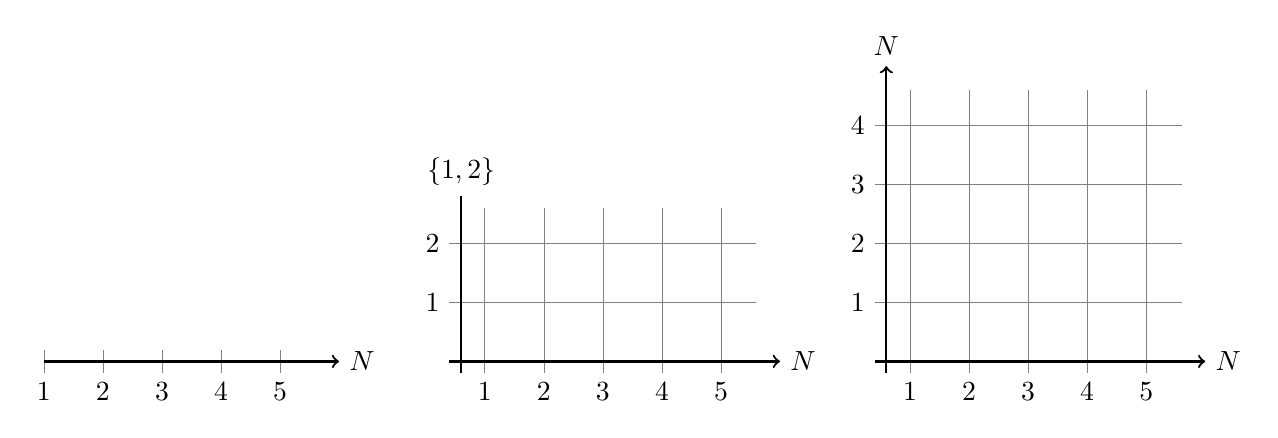
\begin{tikzpicture}
		\begin{scope}[xshift=-5cm,scale=1.5]
			\draw[step=.5cm,style=help lines] (-1,-.1) grid (1.3,.1);
			\draw[->,thick] (-1,0) -- (1.5,0) node[right] {$\mathbb{N}$};
			\foreach \x in {1,2,3,4,5}
				\draw[xshift=.5*\x cm] (-1.5,-.1) node[below] {\x};
		\end{scope}
		
		\begin{scope}[scale=1.5, xshift= 0.4cm]
			\draw[style=help lines,step=.5 cm] (-1.3,-.1) grid (1.3,1.3);
			\begin{scope}
				\draw[->, thick] (-1.3,0) -- (1.5,0) node[right] {$\mathbb{N}$};
				\draw[thick] (-1.2,-.1) -- (-1.2,1.4) node[above] {$\{1,2\}$} coordinate(y axis);
				\foreach \x in {1,2,3,4,5}
					\draw[xshift=.5*\x cm] (-1.5,-.1) node[below] {\x};
				\foreach \y in {1,2}
				\draw[yshift=.5*\y cm] (-1.3,0) node[left] {\y};
			\end{scope}
		\end{scope}
	
		\begin{scope}[scale=1.5,xshift=4cm]
			\draw[style=help lines,step=.5 cm] (-1.3,-.1) grid (1.3,2.3);
			\begin{scope}
				\draw[->, thick] (-1.3,0) -- (1.5,0) node[right] {$\mathbb{N}$};
				\draw[->, thick] (-1.2,-.1) -- (-1.2,2.5) node[above] {$\mathbb{N}$} coordinate(y axis);
				\foreach \x in {1,2,3,4,5}
				\draw[xshift=.5*\x cm] (-1.5,-.1) node[below] {\x};
				\foreach \y in {1,2,3,4}
				\draw[yshift=.5*\y cm] (-1.3,0) node[left] {\y};
			\end{scope}
		\end{scope}
	\end{tikzpicture}
	\centering \caption{Vergleich von $\Nz\cup\Nz=\Nz$, $\Nz\sqcup\Nz$ und $\Nz\times\Nz$.}
\end{figure}

% --------------------------------------------------------------------
% §5 Section <<Übungsaufgaben>>
% --------------------------------------------------------------------


\newpage
\section{Aufgabenvorschläge}

%Bereits bewiesene Sätze (auch aus den vorherigen Vorträgen) dürfen benutzt werden. Es ist euch überlassen, welche Aufgaben ihr die Übungsgruppe rechnen lässt. Ihr solltet die Aufgaben aber vorher einmal selbst gerechnet haben.


% --------------------------------------------------------------------
% §5.1 Subsection <<Elementare Beweise zu Mengenoperationen>>
% --------------------------------------------------------------------





\begin{aufg}[Kennenlernen]
Es sei $T$ die Menge aller Leute, die sich gerade in diesem Tutorium befinden. Welche der folgenden Mengen sind Teilmengen voneinander? Welche Mengen sind sogar gleich?
\begin{align*}
S&:= \{ x\in T \mid x\ \text{ist sportlich} \}  && \emptyset  \\
N&:=  \{ x\in T \mid x\ \text{geht gern in die Natur} \} && T \\
W & := \{ x\in T \mid x\ \text{kennt sich in einem Spezialgebiet richtig gut aus} \} &&  N\setminus S  \\
M &:= \{ x \in T \mid x\ \text{spielt ein Musikinstrument} \} && W \cup S \\
L&:= \{ x\in T \mid x\ \text{ist Single} \} && M\cap L
\end{align*}
\end{aufg}

\begin{comment}
\begin{align*}
 \{x\in \Rz \mid x^3 - 4x = 0 \} &&  \emptyset \\
 \{ n \in \Zz \mid n\ \text{ist eine gerade Zahl} \} &&  \{2\} \\
 \{ x\in \Rz \mid \exists n\in \Zz : n\cdot x \in \Zz \} &&  \{ n\in \Zz \mid \vert n\vert < 4\} \\
 \Nz \setminus \{n\in \Nz \mid n\ \text{ist durch $3$ teilbar} \} &&  \bigcup_{n\in \Nz_{\geq 1}} \left\{ \frac{z}{n} \mid z\in \Zz \right\}
\end{align*}
\end{comment}






\begin{aufg}[Schnitte und Vereinigung konkret]
Für eine natürliche Zahl $n\in\mathbb{N}_0$ sei
\[ M_n:=\{x\in\mathbb{Z}\mid \exists c\in \Zz: c\cdot n = x\} \]
Beweise die folgenden Mengengleichheiten:
\begin{align*}
 & \text{a)} & \bigcap_{n\in\mathbb{N}_0} M_n &= \{0\} \\
 & \text{b)} & \bigcup_{n\in\mathbb{N}_0} M_n & = \mathbb{Z}
 \end{align*}
\end{aufg}






\begin{aufg}[Mengen vs. Familien]
Es sei $I:=\{1,2,3,4,5\}$ und es sei $a=(a_i)_{i\in I}$ diejenige Familie mit $a_i=i+2$ für jedes $i\in I$.
Welche der folgenden Objekte sind einander gleich?
\begin{center}
	{\renewcommand{\arraystretch}{1.6}
		\begin{tabular}{ccccccccc}
		 $I$ && $(a_i)_{i\in I}$&& $\{a_i\mid i\in I\}$ && $(4,3,5,6,7)$ && $(2,1,3,4,5,5)$ \\
		 $a$ && $\{1,2,3,4,5\}$ && $(3,4,5,6,7)$ && $\{4,3,5,6,7\}$ && $\{2,1,3,4,5,5\}$
	\end{tabular}}
\end{center}
\end{aufg}






\begin{aufg}[Produkte konkret]
Wir betrachten die Mengen $T := \{ \text{Dr.} \}, A := \{ \text{Herr, Frau} \}$, $V
:= \{ \text{Anna, Benjamin} \}$ und $N := \{ \text{Hathaway, Sinclair, Wayne}
\}$. Liste die Elemente der folgenden Mengen auf:
\begin{enumerate}[a)]
	\item $A \times N$
%	\item $A \times V \times N$
	\item $A\times T \times V\times N$
	\item $(T \cup V) \times N$
	\item $(T\times N)\cup (V\times N)$
\end{enumerate}
\end{aufg}





\begin{comment}
\begin{aufg}[Teilmengen]
Seien $I$ eine nichtleere Menge, $A,B$ zwei weitere Mengen, sowie $(A_i)_{i\in I}$ eine Familie von Mengen. Mach dir klar, dass die folgenden Teilmengenbeziehungen gelten:\footnote{vgl. dazu \cref{undoderaxiome}, \cref{allaxiom} und \cref{exaxiom}.}
\begin{align*}
 A \cap B & \subseteq A & A & \subseteq A \cup B \\
 A \cap B & \subseteq B & B & \subseteq A \cup B \\
 \forall j\in I:\quad \bigcap_{i\in I}A_i & \subset A_j & \forall j\in I:\quad  A_j & \subseteq \bigcup_{i\in I} A_i \\
 A \cap B & \subseteq A \cup B & \bigcap_{i\in I}A_i & \subset \bigcup_{i\in I}A_i
\end{align*}
\end{aufg}
\end{comment}




\begin{aufg}[Rechenregeln für $\cap$ und $\cup$] \label{capcupgesetze}
Seien $X,Y,Z$ drei beliebige Mengen. Mach dir klar, dass folgende Identitäten gelten:
\begin{align*}
  \begin{split} (X \cap Y) \cap Z & = X \cap (Y \cap Z) \\
  (X \cup Y) \cup Z & = X \cup (Y \cup Z) \end{split} && (\text{Assoziativgesetze}) \\[1em]
  \begin{split} X \cap Y & = Y\cap X \\
  X \cup Y & = Y\cup X
 \end{split} && ( \text{Kommutativgesetze}) \\[1em]
  \begin{split} X \cap (Y \cup Z) & = (X\cap Y) \cup (X\cap Z) \\
   X \cup (Y\cap Z) & = (X\cup Y) \cap (X\cup Z) \end{split} && ( \text{Distributivgesetze}) 
\end{align*}
\end{aufg}





\begin{comment}
\begin{aufg}[Potenzmenge der Potenzmenge der Potenzmenge der \dots]
 Für eine Menge $X$ definieren wir:
 \begin{align*}
  \mathcal{P}^0(X) & := X \\
  \mathcal{P}^1(X) & := \mathcal{P}(X) \\
    \mathcal{P}^2(X) & := \mathcal{P}(\mathcal{P}(X)) \\
      \mathcal{P}^3(X) & := \mathcal{P}(\mathcal{P}(\mathcal{P}(X))) \\
      & \text{usw.}
 \end{align*}
Versuche, die Vereinigungsmenge
\[ \bigcup_{n\in \Nz_0} \mathcal{P}^n(\{1,2,3\}) \]
zu verstehen. Liste acht verschiedene Elemente dieser Menge auf.
\end{aufg}


% --------------------------------------------------------------------
% §5.2 Subsection <<Komplexere Beweise zu Mengenoperationen>>
% --------------------------------------------------------------------


\begin{aufg}[Komplexere Beweise zu Mengenoperationen]
Sei $M$ eine Menge, $A, B \subseteq M$ seien Teilmengen. Zeige:
\begin{enumerate}
\item $M \setminus (M \setminus A) = A$
\item $M \setminus (A\cap B) = (M \setminus A)\cup (M \setminus B)$
\item $M \setminus (A \cup B) = (M \setminus A) \cap (M \setminus B)$
\end{enumerate}
\end{aufg}
\end{comment}
% --------------------------------------------------------------------
% §5.3 Subsection <<Schnitte und Vereinigungen: anschaulich>>
% --------------------------------------------------------------------
\begin{comment}
\begin{aufg}[Schnitte und Vereinigungen: anschaulich]
Zeichne folgende Mengen als Bilder an die Tafel und lass die Studis markierten Bereiche mithilfe der Mengen $A, B$ sowie der bekannten Mengenoperationen angeben:
\begin{enumerate}
\item $A\cap B$
\item $A \setminus B$
\item $(A\setminus B) \cup (B\setminus A)$
\item $A \cup B$ 
\end{enumerate}
\textbf{Alternativ} kannst du sie die Mengen selber zeichnen lassen. Dazu gibst du vorher am besten ein Beispiel, z.B. die erste Menge.
\end{aufg}
\end{comment}

%--------------------------------------------------------------------
% §5.4 Subsection <<Produkte konkret>>
% --------------------------------------------------------------------



% --------------------------------------------------------------------
% §5.4 Subsection <<Schnitte konkret>>
% --------------------------------------------------------------------





\begin{comment}
\begin{aufg}[Kürzbarkeit bezüglich des kartesischen Produkts] Betrachte die folgende Aussage:
 \begin{quote}
  Für alle Mengen $A,B,X$ gilt
  \[ A\times X = B\times X \quad\implies\quad A=B \]
 \end{quote}
 Stimmt das so? Wenn ja, beweise es. Wenn nein, gib ein Gegenbeispiel an.
\end{aufg}
\end{comment}
% --------------------------------------------------------------------
% §5.5 Subsection <<Schnitte und Vereinigungen: Falsche Freunde>>
% --------------------------------------------------------------------
\begin{comment}
\begin{aufg}[Schnitte und Vereinigungen: Falsche Freunde]
Seien $A, B, C$ beliebige Mengen. Unter welchen Bedingungen gilt folgende Aussage:
\begin{align*}
A\cap B = A\cap C \Ra B = C
\end{align*}
\end{aufg}
\end{comment}
% --------------------------------------------------------------------
% §5.6 Subsection <<Mengen vs. Familien>>
% --------------------------------------------------------------------




%%% Local Variables:
%%% mode: latex
%%% TeX-master: "Skript"
%%% End:
